% =====================================================================
% Figure captions for four-column-alignment.tex
%
% Every number quoted below is produced by figures/generate_panels.py,
% which recomputes each quantity from validation/fca.py at plot time
% rather than reading a stored summary. The panels are therefore an
% independent second execution of the framework, not a redraw of the
% validation suite's output. Seed 20260815 throughout; minimum cuts are
% computed exactly by subset enumeration, never approximated.
%
% \input this file, or paste the blocks into the body where wanted.
% =====================================================================

\begin{figure*}[!htbp]
    \centering
    
\includegraphics[width=\textwidth]{figures/panel_1_floor.png}
    \caption{\textbf{The floor: separation cost is bounded below, and the bound survives expansion only conditionally.}
    All quantities are computed on finite weighted graphs with strictly positive edge weights (\Cref{def:fwg}); minimum cuts are exact, obtained by enumeration over all separating vertex subsets rather than by an approximate max-flow routine, so no agreement below can be a solver artefact.
    (\textbf{A})~Distribution of $\sigma(v)/\flo$ over $989$ items drawn from $220$ random contact graphs of $3$--$6$ items. The ratio never falls below $1$ in any instance (minimum exactly $1.000$, median $8.69$, maximum $126.4$), which is \Cref{thm:floor}: the separation cost of an item is at least the contact floor. The mass at the left edge is the set of items whose cheapest cut is the floor edge itself; the long right tail is items embedded in dense neighbourhoods, whose boundary is correspondingly expensive.
    (\textbf{B})~The floor $\flo$ against graph size, median with the $10$--$90$ percentile band over $60$ graphs per size. The median falls monotonically from $0.510$ at three items to $0.117$ at nine, because each additional item contributes further edges and the floor is a minimum over a growing set. It does not reach zero, and cannot: the minimum of a finite set of strictly positive weights is positive (\Cref{thm:floor}). The declining trend and the strict positivity are both essential and are easily conflated, which is why the band rather than the median alone is drawn.
    (\textbf{C})~Mean separation cost as a surface over the number of items and the minimum admissible edge weight, each cell the mean over twelve graphs. The surface rises in both arguments and is bounded away from zero throughout, exhibiting \Cref{thm:floor} as a property of the parameter space rather than of particular instances.
    (\textbf{D})~The local floor $\flo_k(v)$ under three expansion regimes, logarithmic axis. Adding edges at $v$ of weight $1/k$ drives the local floor to $2.5\times10^{-2}$ by step $40$ and $1/k^2$ drives it to $6.3\times10^{-4}$, while a stabilising expansion holds it at $1.0$. This is the content of \Cref{rem:not-positive}: the \emph{unconditional} claim that the intrinsic floor is positive is false, an item can dissolve into the medium in the limit, and \Cref{thm:invariance} is therefore stated under the floor-stabilising hypothesis of \Cref{def:stabilising}. The two decaying curves are the counterexample the theorem must exclude, plotted rather than described.}
    \label{fig:panel1}
\end{figure*}

\begin{figure*}[!htbp]
    \centering
    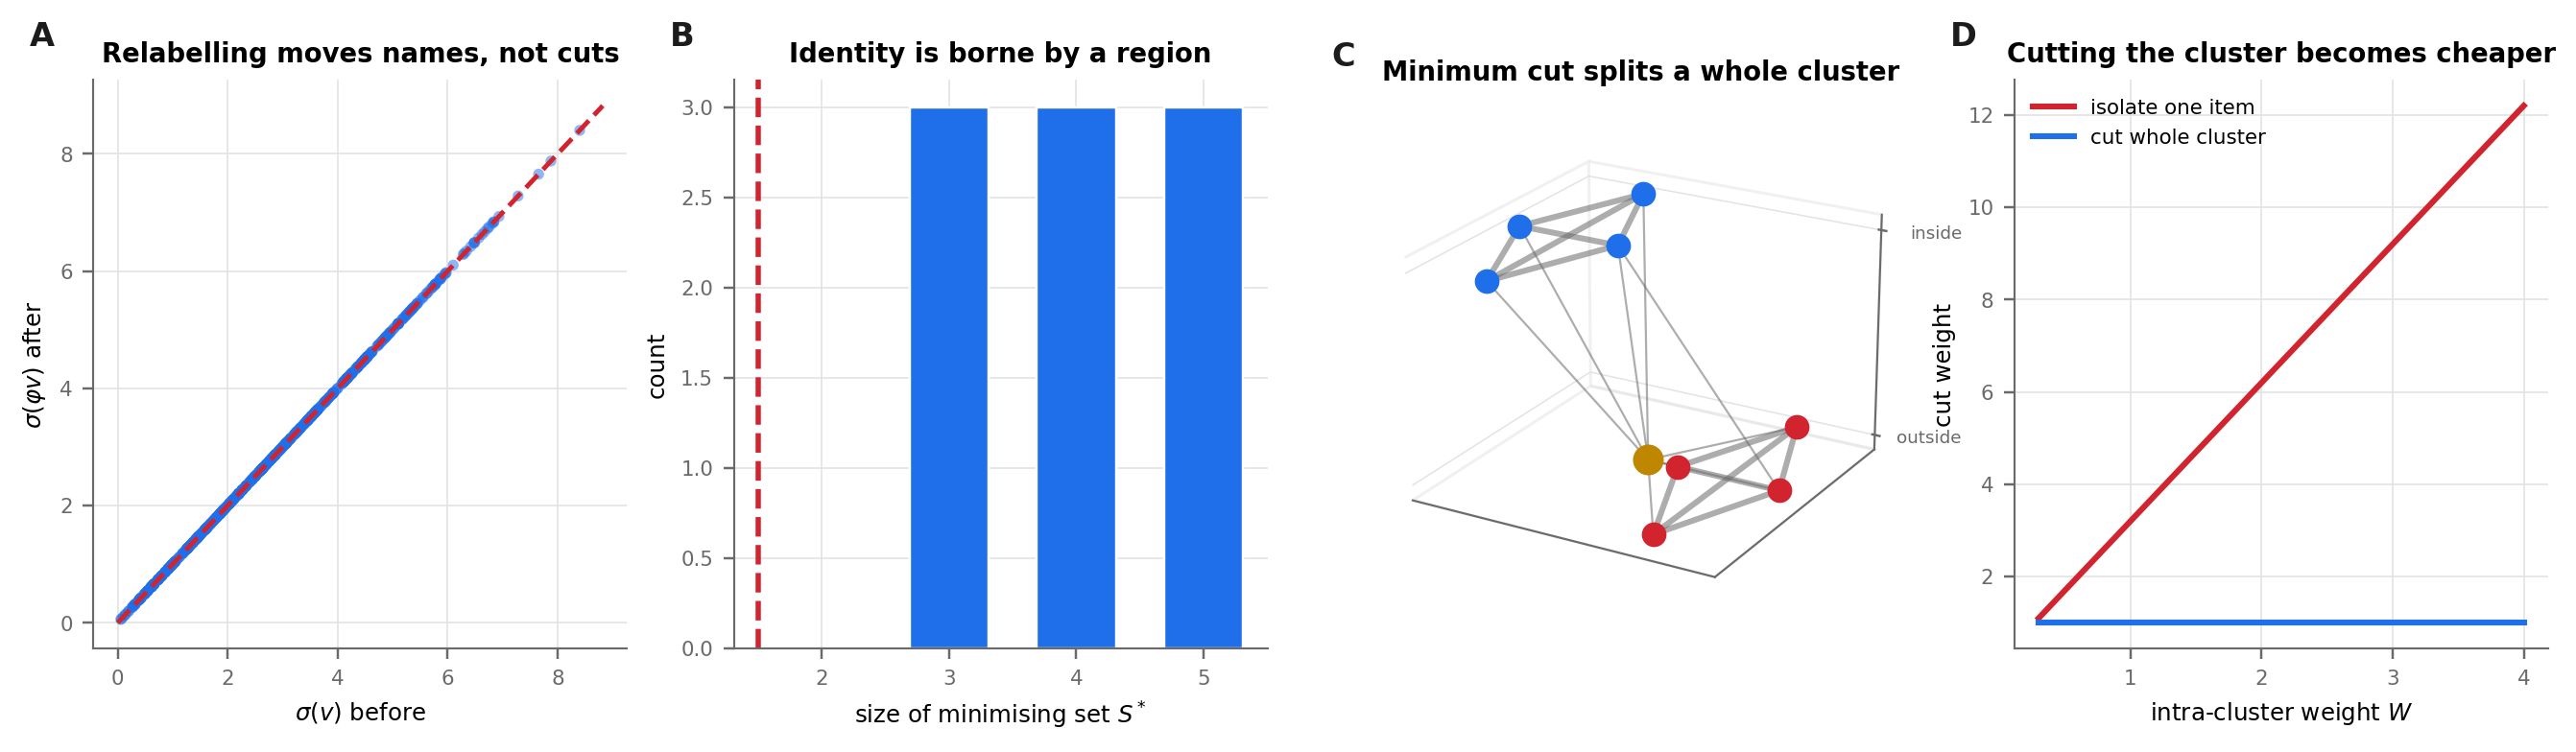
\includegraphics[width=\textwidth]{figures/panel_2_identity.png}
    \caption{\textbf{Identity is an invariant borne by a region of edges, and never by a label or a single vertex.}
    (\textbf{A})~Separation cost before against after a random relabelling, for $727$ items over $160$ graphs. Every point lies on the identity diagonal: the maximum absolute deviation is exactly $0$, not merely small. A weighted isomorphism carries cuts to cuts weight-for-weight, so $\sigma$ is preserved (\Cref{thm:invariant-cut}) while the vertex labels have been permuted --- the invariant and the name come apart, which is \Cref{cor:labels} and, through \Cref{rem:bearing}, the reason a sequence cannot carry what a comparison of sequences is asked to recover.
    (\textbf{B})~Sizes of the minimising set $S^{*}(v)$ over the nine two-cluster instances of the proof of \Cref{thm:region}, spanning $r\in\{3,4,5\}$ and $\flo\in\{0.1,0.2,0.3\}$. Every minimiser has size $3$, $4$ or $5$; none is a singleton (dashed line at $1.5$). The identity of an item is the cut, and the cut in general detaches a whole neighbourhood rather than the item alone.
    (\textbf{C})~One such instance rendered in three dimensions: two four-item clusters joined by a single floor-weight contact, with the medium at the centre (amber). Vertices are lifted by membership of the minimum cut --- inside (blue) against outside (red) --- and edge thickness is proportional to weight. The planar coordinates are an arbitrary layout and carry no quantity, so their ticks are suppressed; only the vertical axis is a measurement. The minimum cut takes the entire left cluster.
    (\textbf{D})~Why it does so. The cost of isolating a single item grows linearly in the intra-cluster weight $W$, since every intra-cluster edge must be severed, while the cost of cutting the whole cluster is flat in $W$, depending only on the medium edges and the single inter-cluster contact. The two curves cross near $W\approx0.5$, and beyond it the region is strictly cheaper than the point. \Cref{rem:badwitness} records that overlooking exactly this --- assuming a light edge between two items places them at the floor --- invalidated our first witness for \Cref{thm:falsefriend}.}
    \label{fig:panel2}
\end{figure*}

\begin{figure*}[!htbp]
    \centering
    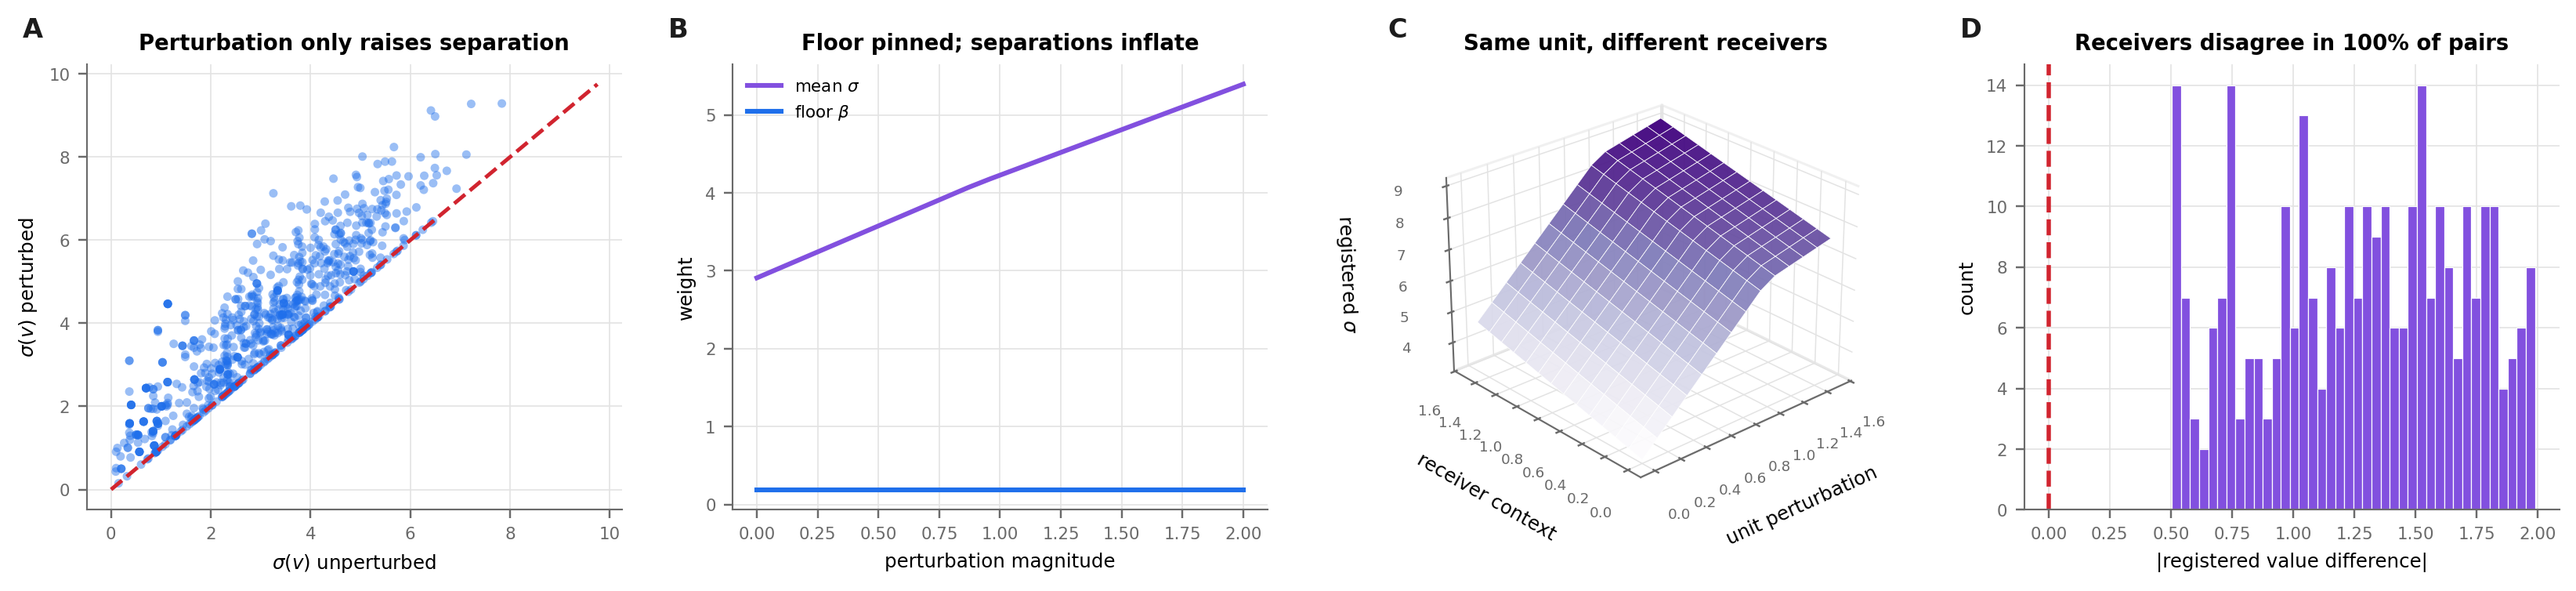
\includegraphics[width=\textwidth]{figures/panel_3_receiver.png}
    \caption{\textbf{Perturbation inflates weights without touching the skeleton, and the value a unit registers depends on the receiver.}
    (\textbf{A})~Separation cost before against after a non-negative perturbation applied to a random subset of edges, over $160$ graphs. Every point lies on or above the diagonal: perturbations raise the cost of distinctions and never lower one, which is the graph-level statement of \Cref{def:perturbation} and the hypothesis \Cref{prop:skeleton} needs. The vertical spread above the diagonal is the inflation itself.
    (\textbf{B})~The floor and the mean separation cost against perturbation magnitude, with the perturbation applied to the heavier half of the edges so that the floor edge is untouched. The mean separation rises from $2.9$ to $5.4$ while the floor stays pinned and the edge count is constant throughout. This is \Cref{prop:skeleton} in its exact form: the edge set is invariant, the weights are not. Perturbing \emph{every} edge would raise the floor as well and would make the same figure say something weaker.
    (\textbf{C})~The registered value $\sigma(v)$ as a surface over two independent axes: the magnitude of the perturbation the unit induces, and the magnitude of an unrelated change to the surrounding network. The surface is not constant along the second axis, so the value a unit registers is a function of the pair (unit, receiver) and not of the unit alone --- \Cref{thm:receiver}.
    (\textbf{D})~The same statement as a distribution. For $300$ pairs of receivers differing only in one background edge, the absolute difference between the values the \emph{same} unit registers is bounded away from zero in every pair. Nothing accumulates at the dashed line at $0$. By \Cref{cor:notnoise} this divergence is not measurement error and is not removed by further assays: the two receivers are evaluating different functions, and each is correct for its own network.}
    \label{fig:panel3}
\end{figure*}

\begin{figure*}[!htbp]
    \centering
    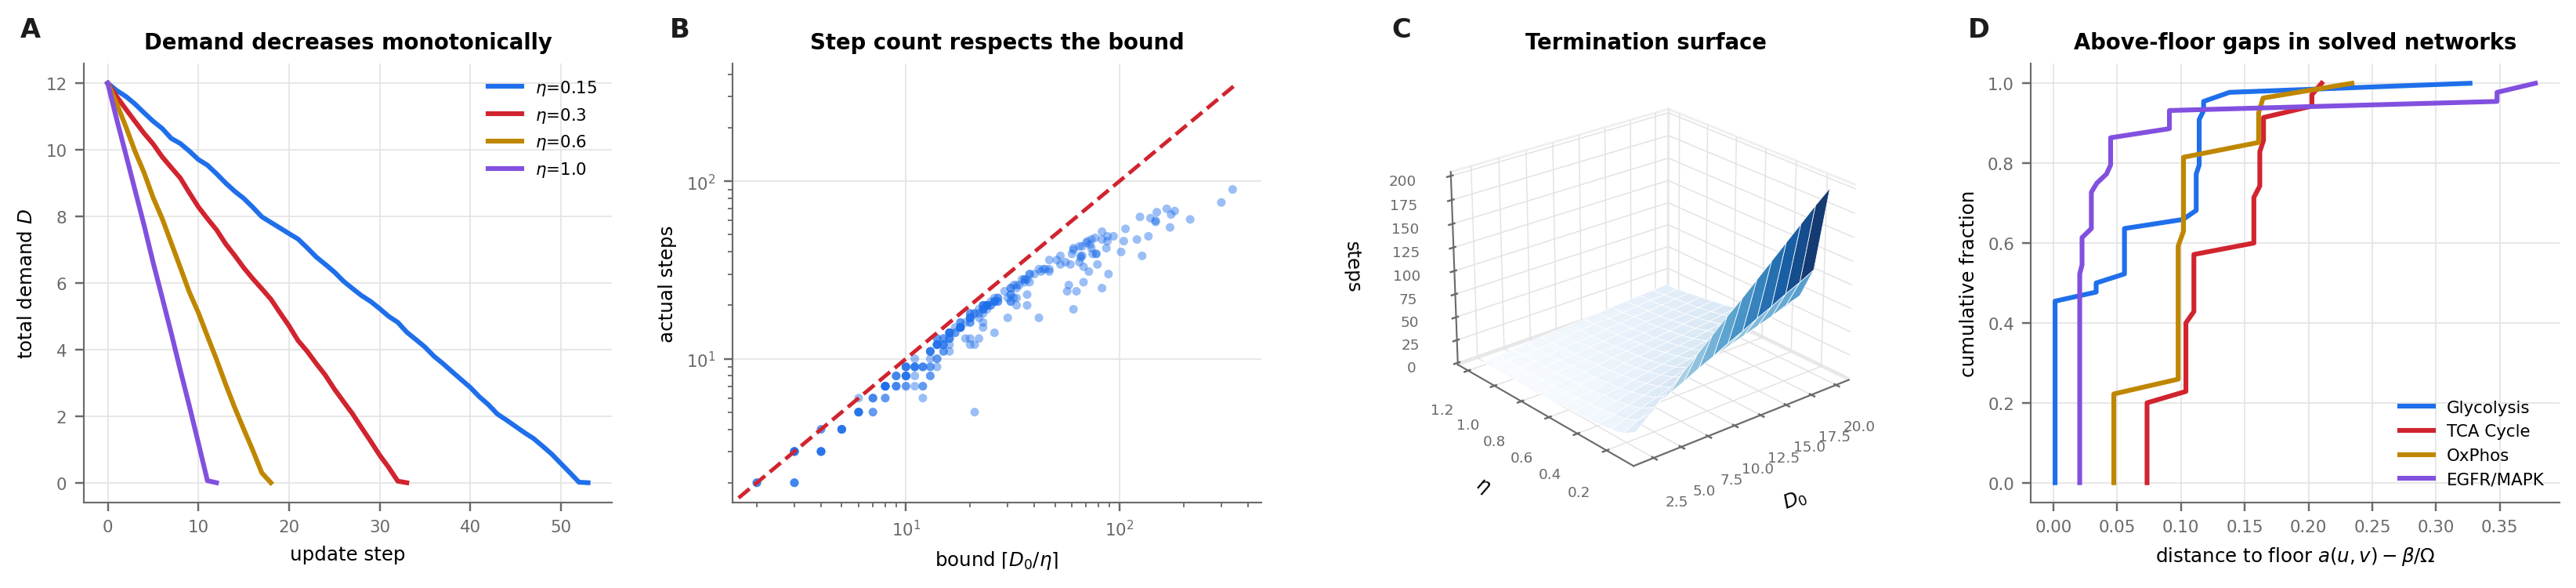
\includegraphics[width=\textwidth]{figures/panel_4_relaxation.png}
    \caption{\textbf{The relaxation decreases monotonically, terminates within the predicted bound, and leaves a positive residual on real networks.}
    (\textbf{A})~Total demand $D$ against update step for four values of the step floor $\eta$. Each trajectory is strictly decreasing to zero, which is \Cref{thm:mono}; larger $\eta$ reaches quiescence in fewer steps. The curves are not smooth because each update decreases $D$ by $\eta$ plus a variable excess, which is what \Cref{ass:effective} permits.
    (\textbf{B})~Realised step count against the bound $\lceil D_0/\eta\rceil$ of \Cref{thm:dichotomy}, for $260$ runs with $D_0$ and $\eta$ drawn independently, both axes logarithmic. Every point lies on or below the diagonal: the bound is never violated and is loose by the accumulated excess. A single point above the line would refute the theorem.
    (\textbf{C})~Step count as a surface over the initial demand $D_0$ and the step floor $\eta$, computed with the excess set to zero so that the surface is the bound itself. It is the graph of $D_0/\eta$, rising steeply as $\eta\to0$: the termination guarantee degrades continuously as updates are permitted to become less effective, and fails only in the limit where \Cref{ass:effective} is abandoned.
    (\textbf{D})~Cumulative distributions of the distance to the floor, $a(u,v)-\flo/\Omega$, over all species pairs in the four solved networks ($45$, $36$, $28$ and $45$ pairs respectively). No pair in any network sits at the floor: the curves leave the origin at zero height. Median gaps are $0.034$ for glycolysis, $0.110$ for the citric-acid cycle, $0.098$ for oxidative phosphorylation and $0.021$ for the EGFR/MAPK cascade. By \Cref{thm:form} this is the expected picture --- quiescence is the vanishing of the \emph{above-floor} excess and coexists with a strictly positive residual, so two systems may place no demand on one another while remaining fully distinguishable.}
    \label{fig:panel4}
\end{figure*}

\begin{figure*}[!htbp]
    \centering
    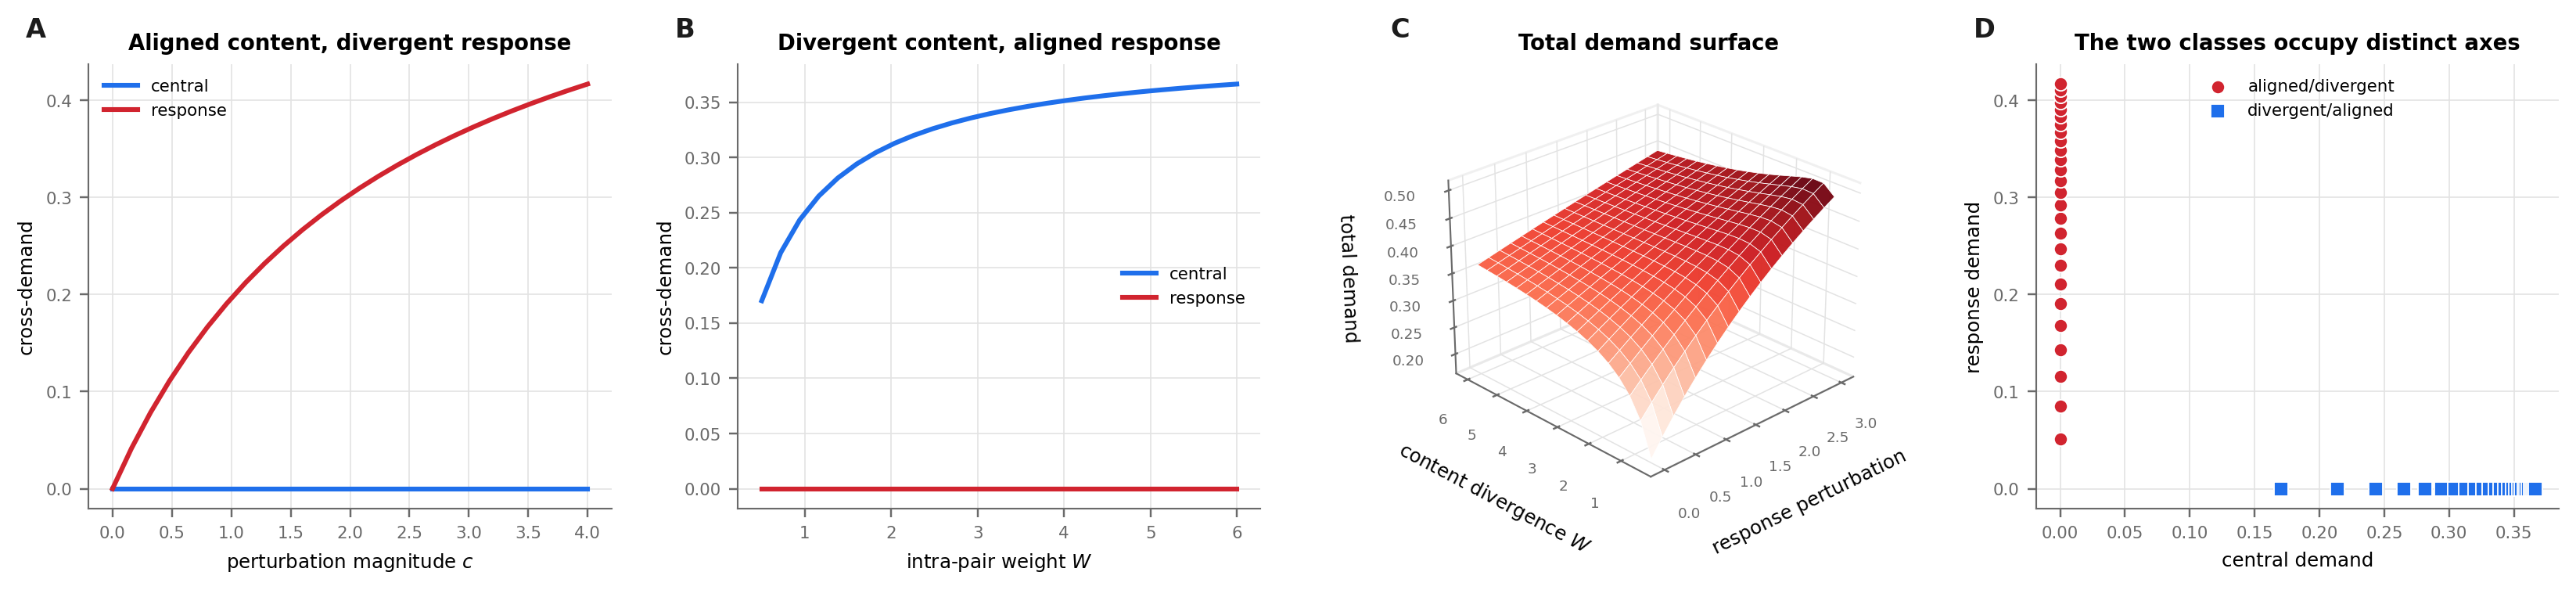
\includegraphics[width=\textwidth]{figures/panel_5_classes.png}
    \caption{\textbf{The two classes that content comparison conflates are separated by the response columns.}
    All four charts use the pendant witness of \Cref{thm:falsefriend} and the two-cluster witness of \Cref{cor:converse}; demands are exact.
    (\textbf{A})~Aligned content with divergent response. As the perturbation magnitude $c$ carried by one unit grows from $0$ to $4$, the central cross-demand stays at exactly $0$ --- the two units are separated at the floor and place no demand on each other --- while the response cross-demand rises to $0.417$. A criterion reading only the central comparison reports correspondence at every value of $c$; the response columns report its absence. This is the synonymous-variant case of \Cref{sec:intro}(i).
    (\textbf{B})~The converse. As the intra-pair weight $W$ grows from $0.5$ to $6$, the central demand rises from $0.170$ to $0.366$ --- the units are increasingly expensive to tell apart --- while the response demand is exactly $0$ throughout, both units inducing the same perturbation. Content comparison reports divergence; the response columns report correspondence. This is the non-homologous isofunctional case of \Cref{sec:intro}(ii).
    (\textbf{C})~Total four-column demand as a surface over both axes at once. The two ridges are the two classes: demand rises along the response axis at fixed content divergence, and along the content axis at fixed response, so neither coordinate alone determines the verdict and \Cref{def:fourq} requires both pairs to be quiescent.
    (\textbf{D})~The two classes in the demand plane. The aligned-content family (circles) lies on the vertical axis at central demand $0$; the divergent-content family (squares) lies on the horizontal axis at response demand $0$. The families are disjoint and occupy orthogonal axes, so a criterion computing only one coordinate necessarily collapses one of them onto the origin. This is the substantive claim of the paper, and it is a geometric fact about the demand plane rather than an empirical tendency.}
    \label{fig:panel5}
\end{figure*}

\begin{figure*}[!htbp]
    \centering
    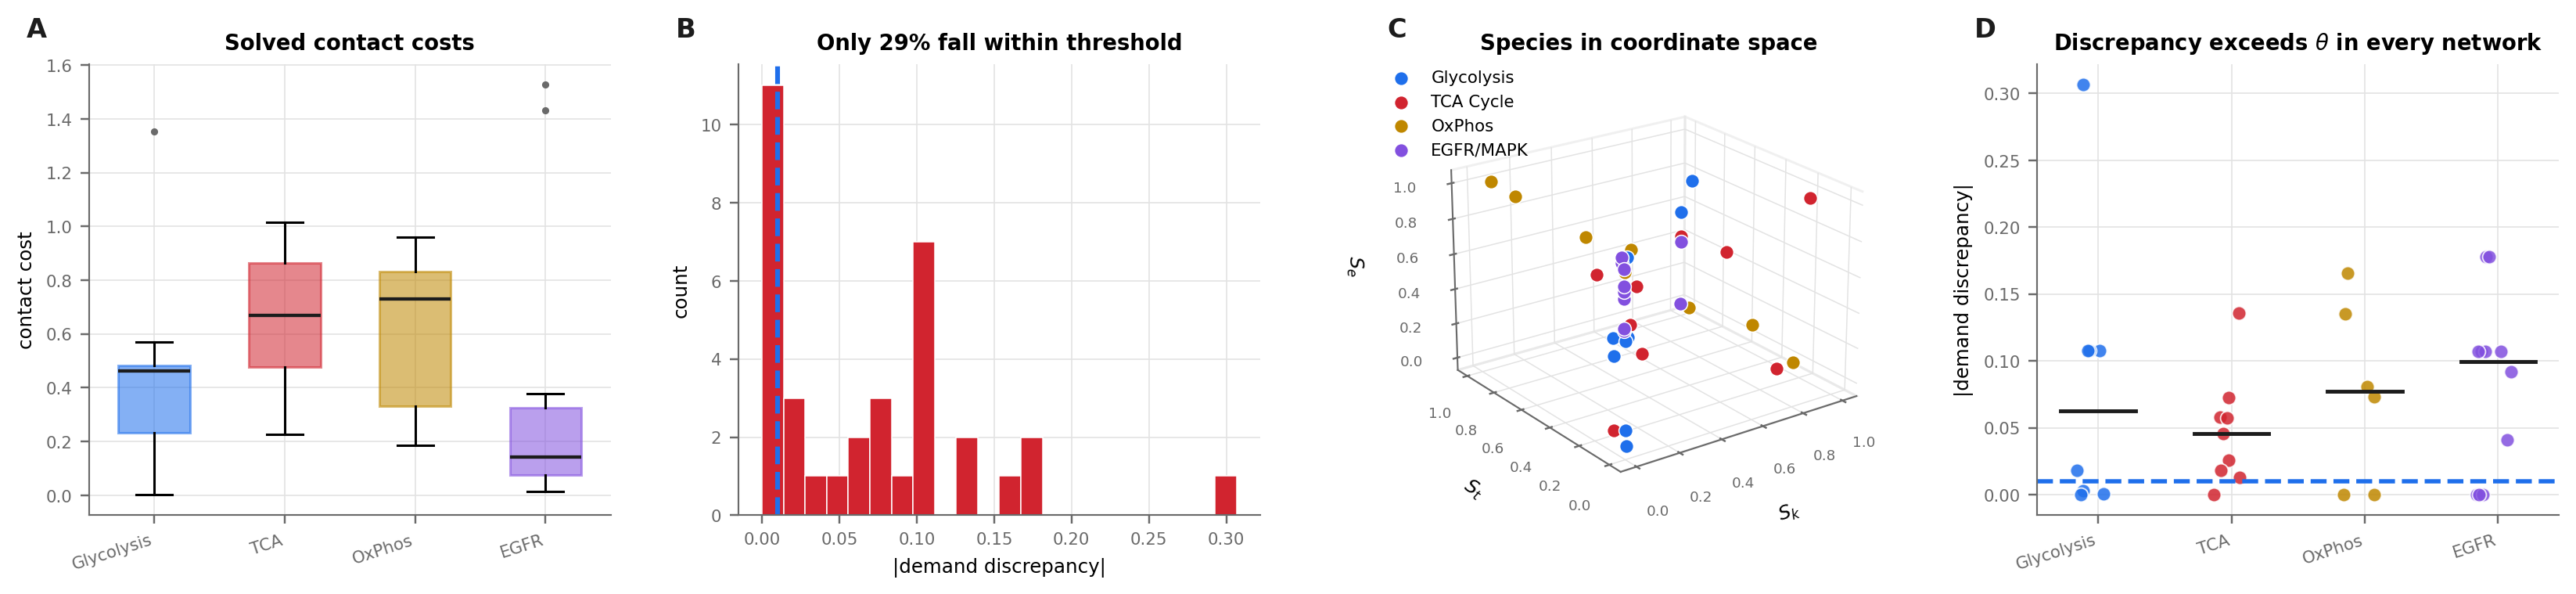
\includegraphics[width=\textwidth]{figures/panel_6_pathways.png}
    \caption{\textbf{On solved biochemical networks the construction is well posed, but response independence fails.}
    Four solved steady-state networks --- glycolysis, the citric-acid cycle, oxidative phosphorylation and the EGFR/MAPK cascade --- supplying $35$ species and $35$ contact edges in total, used here as instances of \Cref{ass:network}.
    (\textbf{A})~Distributions of solved contact cost per network. Costs are strictly positive throughout, so each network is a contact graph in the sense of \Cref{def:contact} and \Cref{thm:floor} applies to it: medians range from $0.141$ for the EGFR/MAPK cascade to $0.729$ for oxidative phosphorylation, with the signalling cascade both the lowest-median and the widest-spread network.
    (\textbf{B})~The decisive measurement of \Cref{con:test}. For each species with at least two incident non-medium edges, two admissible responses are formed by raising one or the other incident edge by the same magnitude, and the resulting cross-demands are compared. Only $28.6\%$ of the $35$ comparisons fall within the decision threshold $\theta=0.01$ (dashed line); the mean discrepancy is $0.070$ and the maximum is $0.307$, exceeding $\theta$ by more than an order of magnitude.
    (\textbf{C})~The $35$ species in the coordinate space of the solved circuits, coloured by network. The four networks occupy overlapping but distinguishable regions; the coordinates are computed from the solved steady state and are shown to establish that the discrepancies of (\textbf{B}) are not an artefact of a degenerate or clustered embedding.
    (\textbf{D})~The same discrepancies resolved by network, with per-network medians as horizontal bars. Every network has a median above $\theta$ --- $0.063$, $0.046$, $0.077$ and $0.100$ respectively --- so the failure is systematic rather than driven by one pathological pathway or one outlying species. By \Cref{prop:respind} the four-column verdict on these networks therefore depends on which admissible response was constructed, and \Cref{ass:respind} does not hold at this threshold. We report this as the framework's principal open problem (\Cref{rem:respind-fails}) rather than as a tuning failure: what is missing is a rule fixing the map from a unit to the perturbation it induces, not better parameters or more data.}
    \label{fig:panel6}
\end{figure*}
